% Experiment 2 (statistics and sweeps): backend/evals/paper/exp2_collusion.py
%   main: 30 seeds per regime; sweeps explore / weight_favours / intensity_adaptive: 10 seeds
Fig.~\ref{fig:z} plots the policy statistic~\eqref{eq:z} for every planted group in the
main runs, under both acceptance models.

\emph{Reading Fig.~\ref{fig:z}.} Each marker is one planted group in one trial. An
open circle is an honest close-knit group and a filled square is a collusion ring.
Each regime has one column: up to 840 honest groups (28 per seed over 30 seeds) and
150 rings (5 per seed). Markers are spread sideways only so that they do not hide one
another; the horizontal position inside a column carries no meaning. The vertical
axis is $z$, how many standard deviations a group's in-group takes lie above what the
acceptance model predicted. At $z=0$ the group did exactly what the model expected;
a positive $z$ means its members took one another's errands more often than
predicted. The horizontal line at $z=3$ is the decision threshold. If the ring search
flags a group below the line, the test clears it; a group above the line goes to a
reviewer. The two numbers above each column count the honest groups (top) and rings
(bottom) on or above the line. A good test puts the circles below the line and the
squares above it. Panel (a) does this in the routine and busy regimes but not with
coordinated rings, whose squares sit among the circles. In panel (b) those squares
rise above the line while the circles stay near zero. In the favours and hard
columns, many circles cross the line in both panels: honest groups that deliberately
route favours look like rings to any test built on these logs.

\emph{Calibration.} With the router's scores (Fig.~\ref{fig:z}(a)), honest groups in
the routine regime had a median $z$ of $-2.1$: the router's scores predict more
in-group takes than honest groups make, because every candidate in a tier is told at
once and the order of the list matters little. The fitted model
(Fig.~\ref{fig:z}(b)) centres honest groups near zero (median $-0.2$), which is what
a calibrated test should do. Its weights describe the simulated behaviour as one would
hope: averaged over seeds, a kilometre of distance cost 0.65 in log-odds and being a
direct friend added 0.51, rising to 0.97 in the busy regime, where friends were
simulated as four times likelier to accept. Friend-of-friend status added almost
nothing ($-0.03$), and reputation is constant in the simulation, so its weight is
zero.

\emph{Separation.} In the routine and busy regimes both versions separated cleanly:
every ring and at most 1\% of honest groups reached $z=3$. Against coordinated rings
they part ways. With the router's scores only 3 of 150 rings reached the line (median
$z=0.4$), because a partner who is always the router's first pick looks, to a test
that trusts the router, like the router's own doing. With the fitted model 112 of 150
did (median 3.7). A friend who takes a group's errands every time is unusual compared
with how friends elsewhere on campus behave, and that comparison is what the fitted
model makes.

\emph{Honest favours.} When honest groups deliberately route favours to each other,
34\% of them exceeded $z=3$ under the router's scores and 42\% under the fitted model,
because the fitted model no longer starts from a conservative margin. The test only
acts on groups the ring search raised, though, and of the 50 honest-only cycles
raised in the favours regime it cleared 35 (the router-score version cleared 37).

\begin{figure}[!t]
\centering
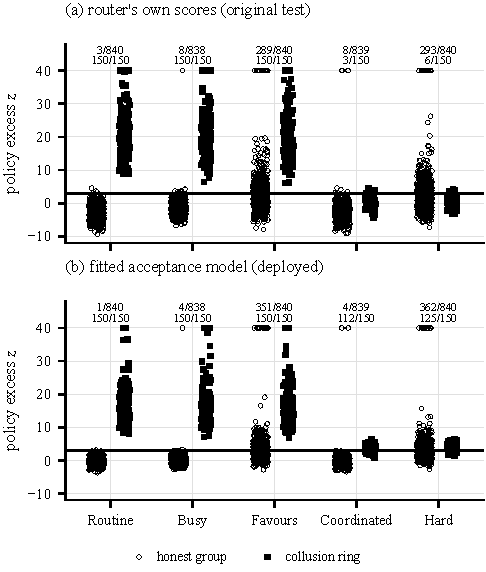
\includegraphics[width=\columnwidth]{figures/fig_z.pdf}
\caption{Policy statistic $z$ for every planted group in the main runs (30 seeds per
regime; 28 honest groups and 5 rings per seed) under (a) the router's own logged scores
and (b) the fitted acceptance model. Numbers above each column count honest groups
(top) and rings (bottom) with $z\ge3$, which the test does not clear. Values above 40,
including the $\pm99$ of the degenerate case, are drawn at 40.}
\label{fig:z}
\end{figure}

\emph{Exploration.} Fig.~\ref{fig:explore} varies the exploration rate, ten seeds per
point. The router-score test needed exploration to see coordinated rings at all: its
recall was 0.03 at the deployed 5\%, 0.38 at 20\% and 0.88 at 40\%. The fitted test did
not. Its recall was 0.84 with no exploration, 0.86 at 5\% and 0.98 at 40\%, because it
learns from variation across the whole campus, not from the exploratory rounds of the
group under test. In the busy regime both versions held false positives under one
honest student per trial at every rate, against 1.1 to 3.8 for the ring search alone.
Since exploration costs service (Section~\ref{sec:eval-dispatch}), the fitted model
removes the main reason to raise it.

\emph{Reading Fig.~\ref{fig:explore}.} The horizontal axis of both panels is the
exploration rate, the share of first offers sent without the social boost; the dotted
vertical line marks the deployed 5\%. Panel (a) measures recall against coordinated
rings: the share of the 26 ring members still flagged after the policy test. The
dashed line with open circles is the ring search alone, an upper bound, because the
test can only remove flags, never add them. The dotted line with triangles is the
original test, using the router's scores, and the solid line with filled squares is
the deployed test, using the fitted model. The vertical gap between the dashed line
and a test's line is the share of ring members that test wrongly cleared. The
original test closes that gap only at 40\% exploration; the fitted test stays close
to it at every rate. Panel (b) counts honest students falsely flagged per trial in
the busy regime, where the router itself puts honest friends together, so lower is
better. Here the dashed line shows how many flags the router causes, and the two test
lines show how many remain. Each point is the mean over ten seeds, and its error bar
is the 95\% confidence interval of that mean. The bars in panel (b) are wide because
false positives are few and vary from seed to seed between zero and a handful.

\begin{figure}[!t]
\centering
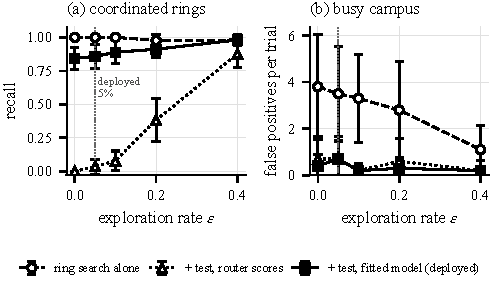
\includegraphics[width=\columnwidth]{figures/fig_explore.pdf}
\caption{Effect of the exploration rate. (a) Recall against coordinated rings. (b)
Honest students falsely flagged per trial in the busy regime. Mean and 95\% confidence
interval over ten seeds; the dotted line marks the deployed rate.}
\label{fig:explore}
\end{figure}

\emph{Trust weight.} The trust weight in~\eqref{eq:effective} changed nothing about
who accepted in our simulation: in-group shares and ring-search results were identical
at 0, 1500 and 3000~m, because every runner in a tier is told at the same moment. It
did change what the router-score test expected. With the weight at zero that test kept
97\% of coordinated ring members flagged, and at 1500 or 3000~m it kept 3\%. The fitted
test kept 86\% at all three weights, because it never reads the router's weights.

\emph{The two limits.} Fig.~\ref{fig:sweeps} shows where relational evidence stops.
As honest groups trade more favours (panel a), the ring search flags more of them:
0.1, 1.9, 7.8, 37.6 and 112.6 honest students per trial at 0, 3, 6, 12 and 24 favours
per member. The fitted test cleared 63\% of these at three favours per member and 76\%
at six, but only 27\% at twelve and 2\% at twenty-four. That much deliberate in-group
routing is beyond what ordinary friends do, and the test is right to say so; what it
cannot say is that the routing was innocent. Panel (b) shows the other end. Because a
leg must carry at least five errands or Rs.~150, and honest runners sometimes take a
ring's errand first, the ring search found almost no ring member when rings farmed
four or fewer errands per member in a semester, 47\% at eight and 97\% at twelve. The
\emph{adaptive} attacker, a coordinated ring that chooses how much to farm, adds the
policy test's own floor: against it the deployed pipeline caught 42\% of members at
eight errands, 86\% at twelve and all of them at twenty-four. Below that floor the
pipeline is blind, but the farming is also small: at four errands per member the five
rings together moved about Rs.~1,600 in a semester, and under one vote per rater a
member farming from three partners gets three votes however many errands they run
(Section~\ref{sec:eval-farming}).

\emph{Reading Fig.~\ref{fig:sweeps}.} In panel (a) the horizontal axis is the number
of favours each honest group member deliberately routes to a friend in a semester,
and the vertical axis is the number of honest students flagged per trial. The three
lines use the same markers as Fig.~\ref{fig:explore}. The gap between the dashed line
(ring search alone) and the solid line (deployed test) is the honest flags that the
test clears. That gap is wide at three and six favours, narrows at twelve and all but
closes at twenty-four, where the lines meet: there the test, correctly by its own
definition, finds the routing unexplained. In panel (b) the horizontal axis is the
number of farmed errands per ring member in a semester, and the vertical axis is
recall. The dashed line is careless (routine) rings against the ring search alone;
where it rises shows the qualification floor of a payment leg. The solid line is
coordinated rings, which choose their own volume, against the deployed pipeline;
where it rises shows how much an adaptive ring can farm before it is caught. The
point where a curve leaves zero is the volume a ring can stay under. Error bars are
95\% confidence intervals over ten seeds; they are widest at eight errands, where
whether a ring is caught depends on chance in individual seeds.

\begin{figure}[!t]
\centering
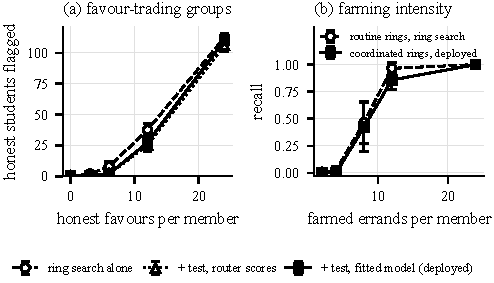
\includegraphics[width=\columnwidth]{figures/fig_sweeps.pdf}
\caption{(a) Honest students flagged as honest favour-trading grows (legend below).
(b) Recall as rings farm fewer errands: careless rings against the ring search, and
coordinated rings, which choose their volume, against the deployed pipeline. Mean and
95\% confidence interval over ten seeds.}
\label{fig:sweeps}
\end{figure}
